\documentclass[nobinding]{sydeStyle}	% use this line for design reports that are not going to be bound
%\documentclass{sydeStyle}		% use this line for design reports that are going to be bound
%\documentclass[workreport]{sydeStyle}	% use this line for work reports (always bound)

\usepackage{longtable}
\usepackage{rotating}
\usepackage{multirow}
\usepackage{amsmath, amsthm, SIunits}


\begin{document}
% SyDe report titlepage
\title{report title}
\coursecode{123}
\labinfo{Wednesday Lab: Station 1}
\author{name, student id, term}
\authortwo{name, student id, term}
\authorthree{name, student id, term}
\authorfour{name, student id, term}
\date{October 22, 2006}
\prof{Professor A. Smithee}
\maketitle


\cleardoublepage
\pagenumbering{roman}

\setcounter{page}{2} % the table of contents will be shown as page ii
\tableofcontents
\addcontentsline{toc}{chapter}{\hspace{13pt} Contents}

\listoftables
\addcontentsline{toc}{chapter}{\hspace{13pt} List of Tables}

\listoffigures
\addcontentsline{toc}{chapter}{\hspace{13pt} List of Figures}

\cleardoublepage
\pagenumbering{arabic}


\chapter{Sample Chapter}%
	\section{Sample Section}
Lorem ipsum dolor sit amet, consectetuer adipiscing elit. Curabitur vulputate dui id justo. Etiam vitae nunc a tortor gravida lobortis. Etiam pretium dignissim erat. Donec gravida placerat ligula. Pellentesque sed mauris. Cum sociis natoque penatibus et magnis dis parturient montes, nascetur ridiculus mus. Pellentesque pharetra mattis ipsum. Class aptent taciti sociosqu ad litora torquent per conubia nostra, per inceptos hymenaeos. Nunc porttitor sem eu enim. Aliquam sem eros, vulputate id, vehicula eu, tristique vel, purus. Nullam et erat id eros semper porttitor. Etiam ultrices molestie risus. Nunc gravida. Curabitur ultricies. Aliquam nec sem.

Suspendisse a lacus. Etiam gravida. Ut elementum tortor non est. Suspendisse ligula orci, porta eget, aliquet et, commodo ut, ligula. Vivamus in nisi non justo convallis congue. Aliquam erat volutpat. Integer sodales luctus metus. Fusce nisl. Aenean at lacus et felis pulvinar sodales. In imperdiet, est a vehicula tincidunt, turpis eros venenatis ante, id tincidunt ligula est a lacus. In hac habitasse platea dictumst. Nulla lorem urna, lacinia a, pellentesque eget, sodales ut, nisl. Duis rutrum interdum urna. Integer ullamcorper libero ut risus. Suspendisse cursus lectus vel ante. Quisque massa metus, aliquam nec, fringilla nec, commodo id, diam. Proin tristique tortor vitae leo. Nulla urna.
	\subsection{Sample Subsection}
Lorem ipsum dolor sit amet, consectetuer adipiscing elit. Curabitur vulputate dui id justo. Etiam vitae nunc a tortor gravida lobortis. Etiam pretium dignissim erat. Donec gravida placerat ligula. Pellentesque sed mauris. Cum sociis natoque penatibus et magnis dis parturient montes, nascetur ridiculus mus. Pellentesque pharetra mattis ipsum. Class aptent taciti sociosqu ad litora torquent per conubia nostra, per inceptos hymenaeos. Nunc porttitor sem eu enim. Aliquam sem eros, vulputate id, vehicula eu, tristique vel, purus. Nullam et erat id eros semper porttitor. Etiam ultrices molestie risus. Nunc gravida. Curabitur ultricies. Aliquam nec sem.

Suspendisse a lacus. Etiam gravida. Ut elementum tortor non est. Suspendisse ligula orci, porta eget, aliquet et, commodo ut, ligula. Vivamus in nisi non justo convallis congue. Aliquam erat volutpat. Integer sodales luctus metus. Fusce nisl. Aenean at lacus et felis pulvinar sodales. In imperdiet, est a vehicula tincidunt, turpis eros venenatis ante, id tincidunt ligula est a lacus. In hac habitasse platea dictumst. Nulla lorem urna, lacinia a, pellentesque eget, sodales ut, nisl. Duis rutrum interdum urna. Integer ullamcorper libero ut risus. Suspendisse cursus lectus vel ante. Quisque massa metus, aliquam nec, fringilla nec, commodo id, diam. Proin tristique tortor vitae leo. Nulla urna.

\chapter{Figures, Tables \& Equations}
\section{A Sample Figure}
		\begin{figure}[h]
			\begin{center}
			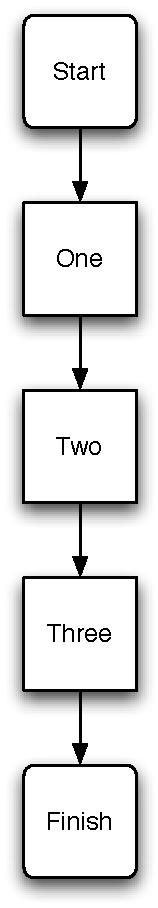
\includegraphics[height=.5\textheight]{flow}
			\caption{A Sample Flowchart}
			\label{results}
			\end{center}
		\end{figure}

\section{Sample Tables}
\begin{table}[h]
	\begin{tabular}{|c||ccc|}
		\hline
	\textbf{\em k}  &  $x_1^k$    &   $x_2^k$  & $x_3^k$ \\
		\hline \hline
	0   & -0.30000000 & 0.60000000 & ~0.70000000 \\
	1   & ~0.47102965 & 0.04883157 & -0.53345964 \\
	2   & ~0.49988691 & 0.00228830 & -0.52246185 \\
	3   & ~0.49999976 & 0.00005380 & -0.52365600 \\
	4   & ~0.50000000 & 0.00000307 & -0.52359743 \\
		\hline
	7   & ~0.50000000 & 0.00000000 & -0.52359878 \\
		\hline
	\end{tabular}
	\caption{A Sample Table Full Of Nonsense Data}
\end{table}

\section{Sample Equations}
\textit{The Relationship Between Acceleration and the Coefficients of Friction}
\begin{align*}
\sum F & = m\vec{a}\\
& = \vec{F_{F}}+\vec{w}\\
& = \mu(-\vec{w}\cos{\theta}) + \vec{w}\sin{\theta}\\
& = \vec{w}(\sin{\theta} - (\cos{\theta})\mu)\\
m\vec{a} & = m\vec{g}(\sin{\theta} - (\cos{\theta})\mu)\\
\vec{a} & = \vec{g}(\sin{\theta} - (\cos{\theta})\mu)\\
\end{align*}


\end{document}
